\chapter{Frontend} \label{chap:Frontend}
One of the primary goals of this application to give the lecturer a way to specify what constitutes a correct problem solution.
As previously mentioned in the \textbf{Use Cases} section of chapter \ref{chap:Specification}, a common approach to this is the use of test cases.

\section{Authentication and Roles}
When a user initially loads the frontend website, they will not be signed in, and will will only have minimal privileges.
This means that they will not have access to any of the course material or exercises.
In order to access any of these features, the user has to sign in.
By pressing the sign in button, the user is redirected to a sign in page that is specific to the authentication provider used.
In our case, it is Google.
After logging in with the authentication provider, the user is redirected back to the website.
At this point, the user is now logged in and our database will be updated with the user's information, as well as a token to keep track of the user's session.
This token is used by NextAuth to create a session for the user, which will be used to authenticate the user for subsequent requests to the site.
The session also has a role associated with it, which determines what actions the user is allowed to take on the site.
Figure \ref{fig:Home page} shows the landing page after the user has signed in. As can be seen, the \texttt{Courses} and \texttt{Dashboard} buttons on the navigation bar is available.
\begin{figure}[H]
    \centering
    \frame{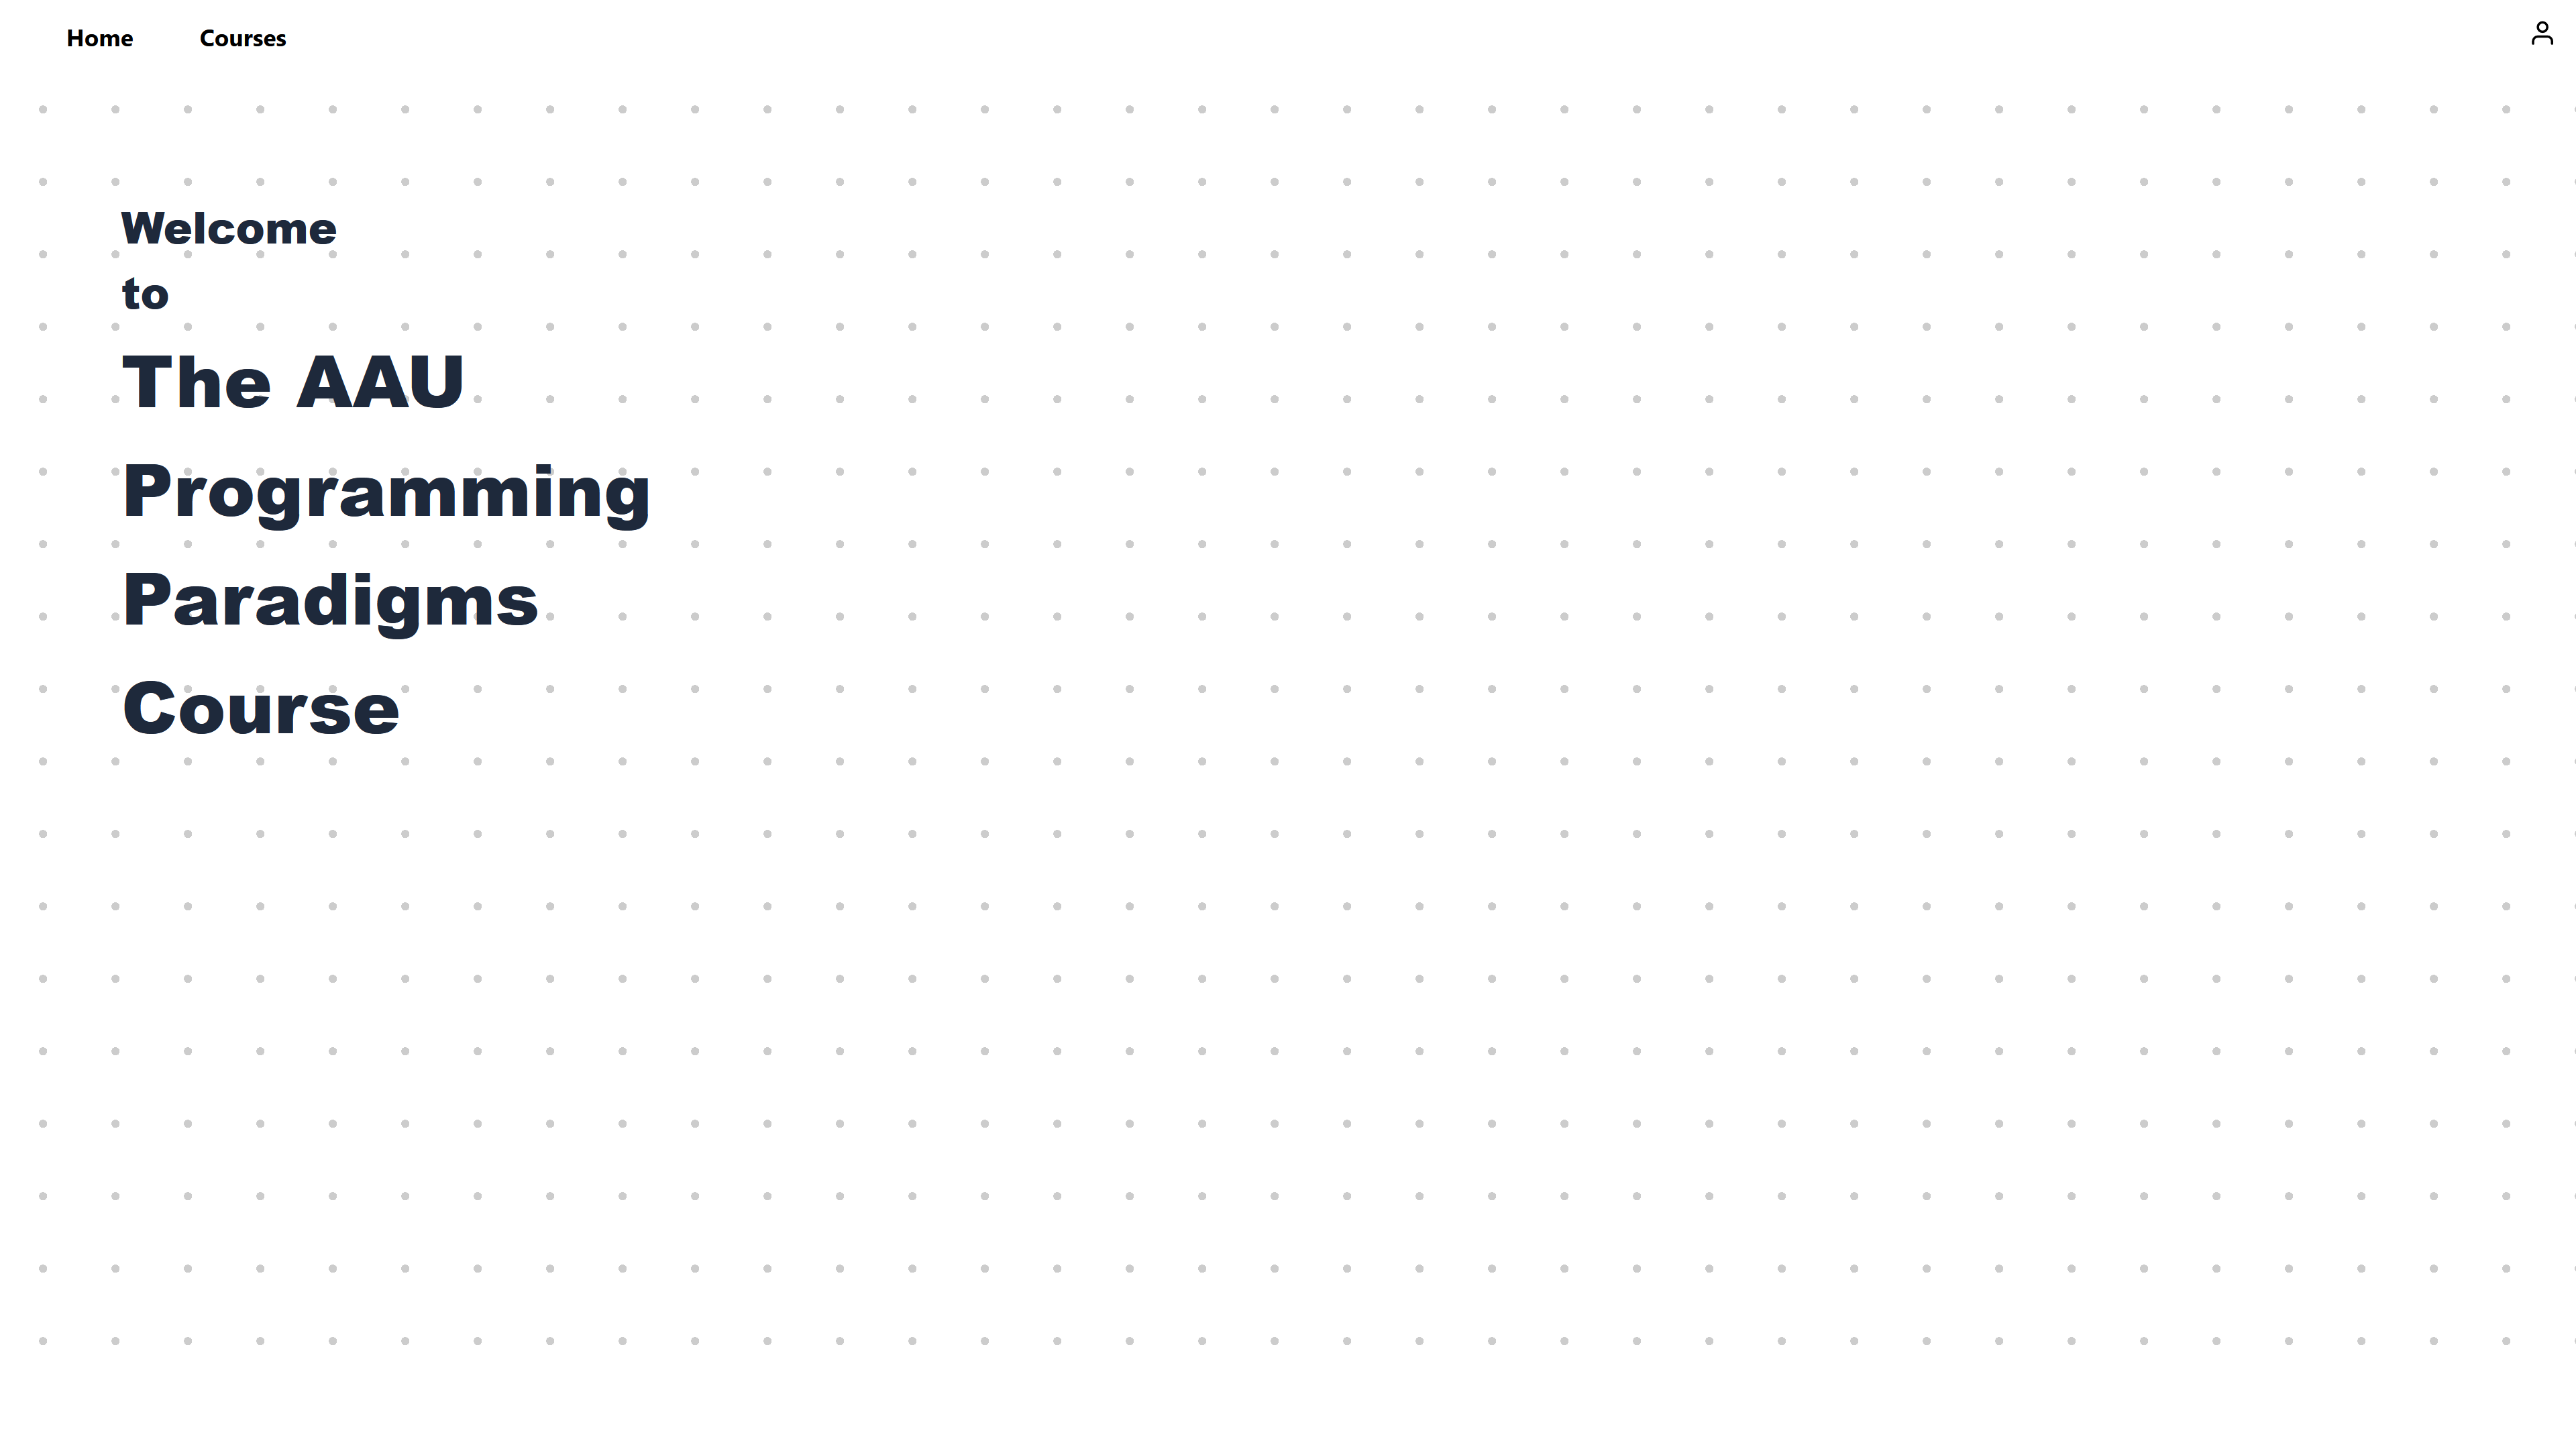
\includegraphics[scale=0.1]{home.png}}
    \caption{Home page as a logged-in user}
    \label{fig:Home page}
\end{figure}

\section{Syllabi, Problem sets and Exercises}
On the website, each page that displays course data makes a request to a Next.js backend API endpoint to retrieve the data from the database.
This request is made using tRPC, which allows for efficient communication between the frontend and the backend. tRPC wraps around React Query, which provides useful features such as caching and automatic refetching.
The request input is validated  ensure that it is in the correct format.
The user's authorization is also checked to ensure that they are allowed to access the data they have requested.
Once the input has been validated, the database is queried using Prisma to retrieve the requested data.

The actions that a user is allowed to take on a page depend on their role. For example, a lecturer may have the ability to create, edit, and delete syllabi, problem sets, and exercises, whereas a student may only be able to read the information on the page.

There is a modal on the page that contains form controls for creating new elements, such as syllabi or problem sets.
This modal helps to prevent invalid input by ensuring that the user enters the correct information before creating a new element.
Overall, our website supports create, read, update, and delete actions for lecturers and read-only access for students.

\begin{figure}[H]
    \centering
    \frame{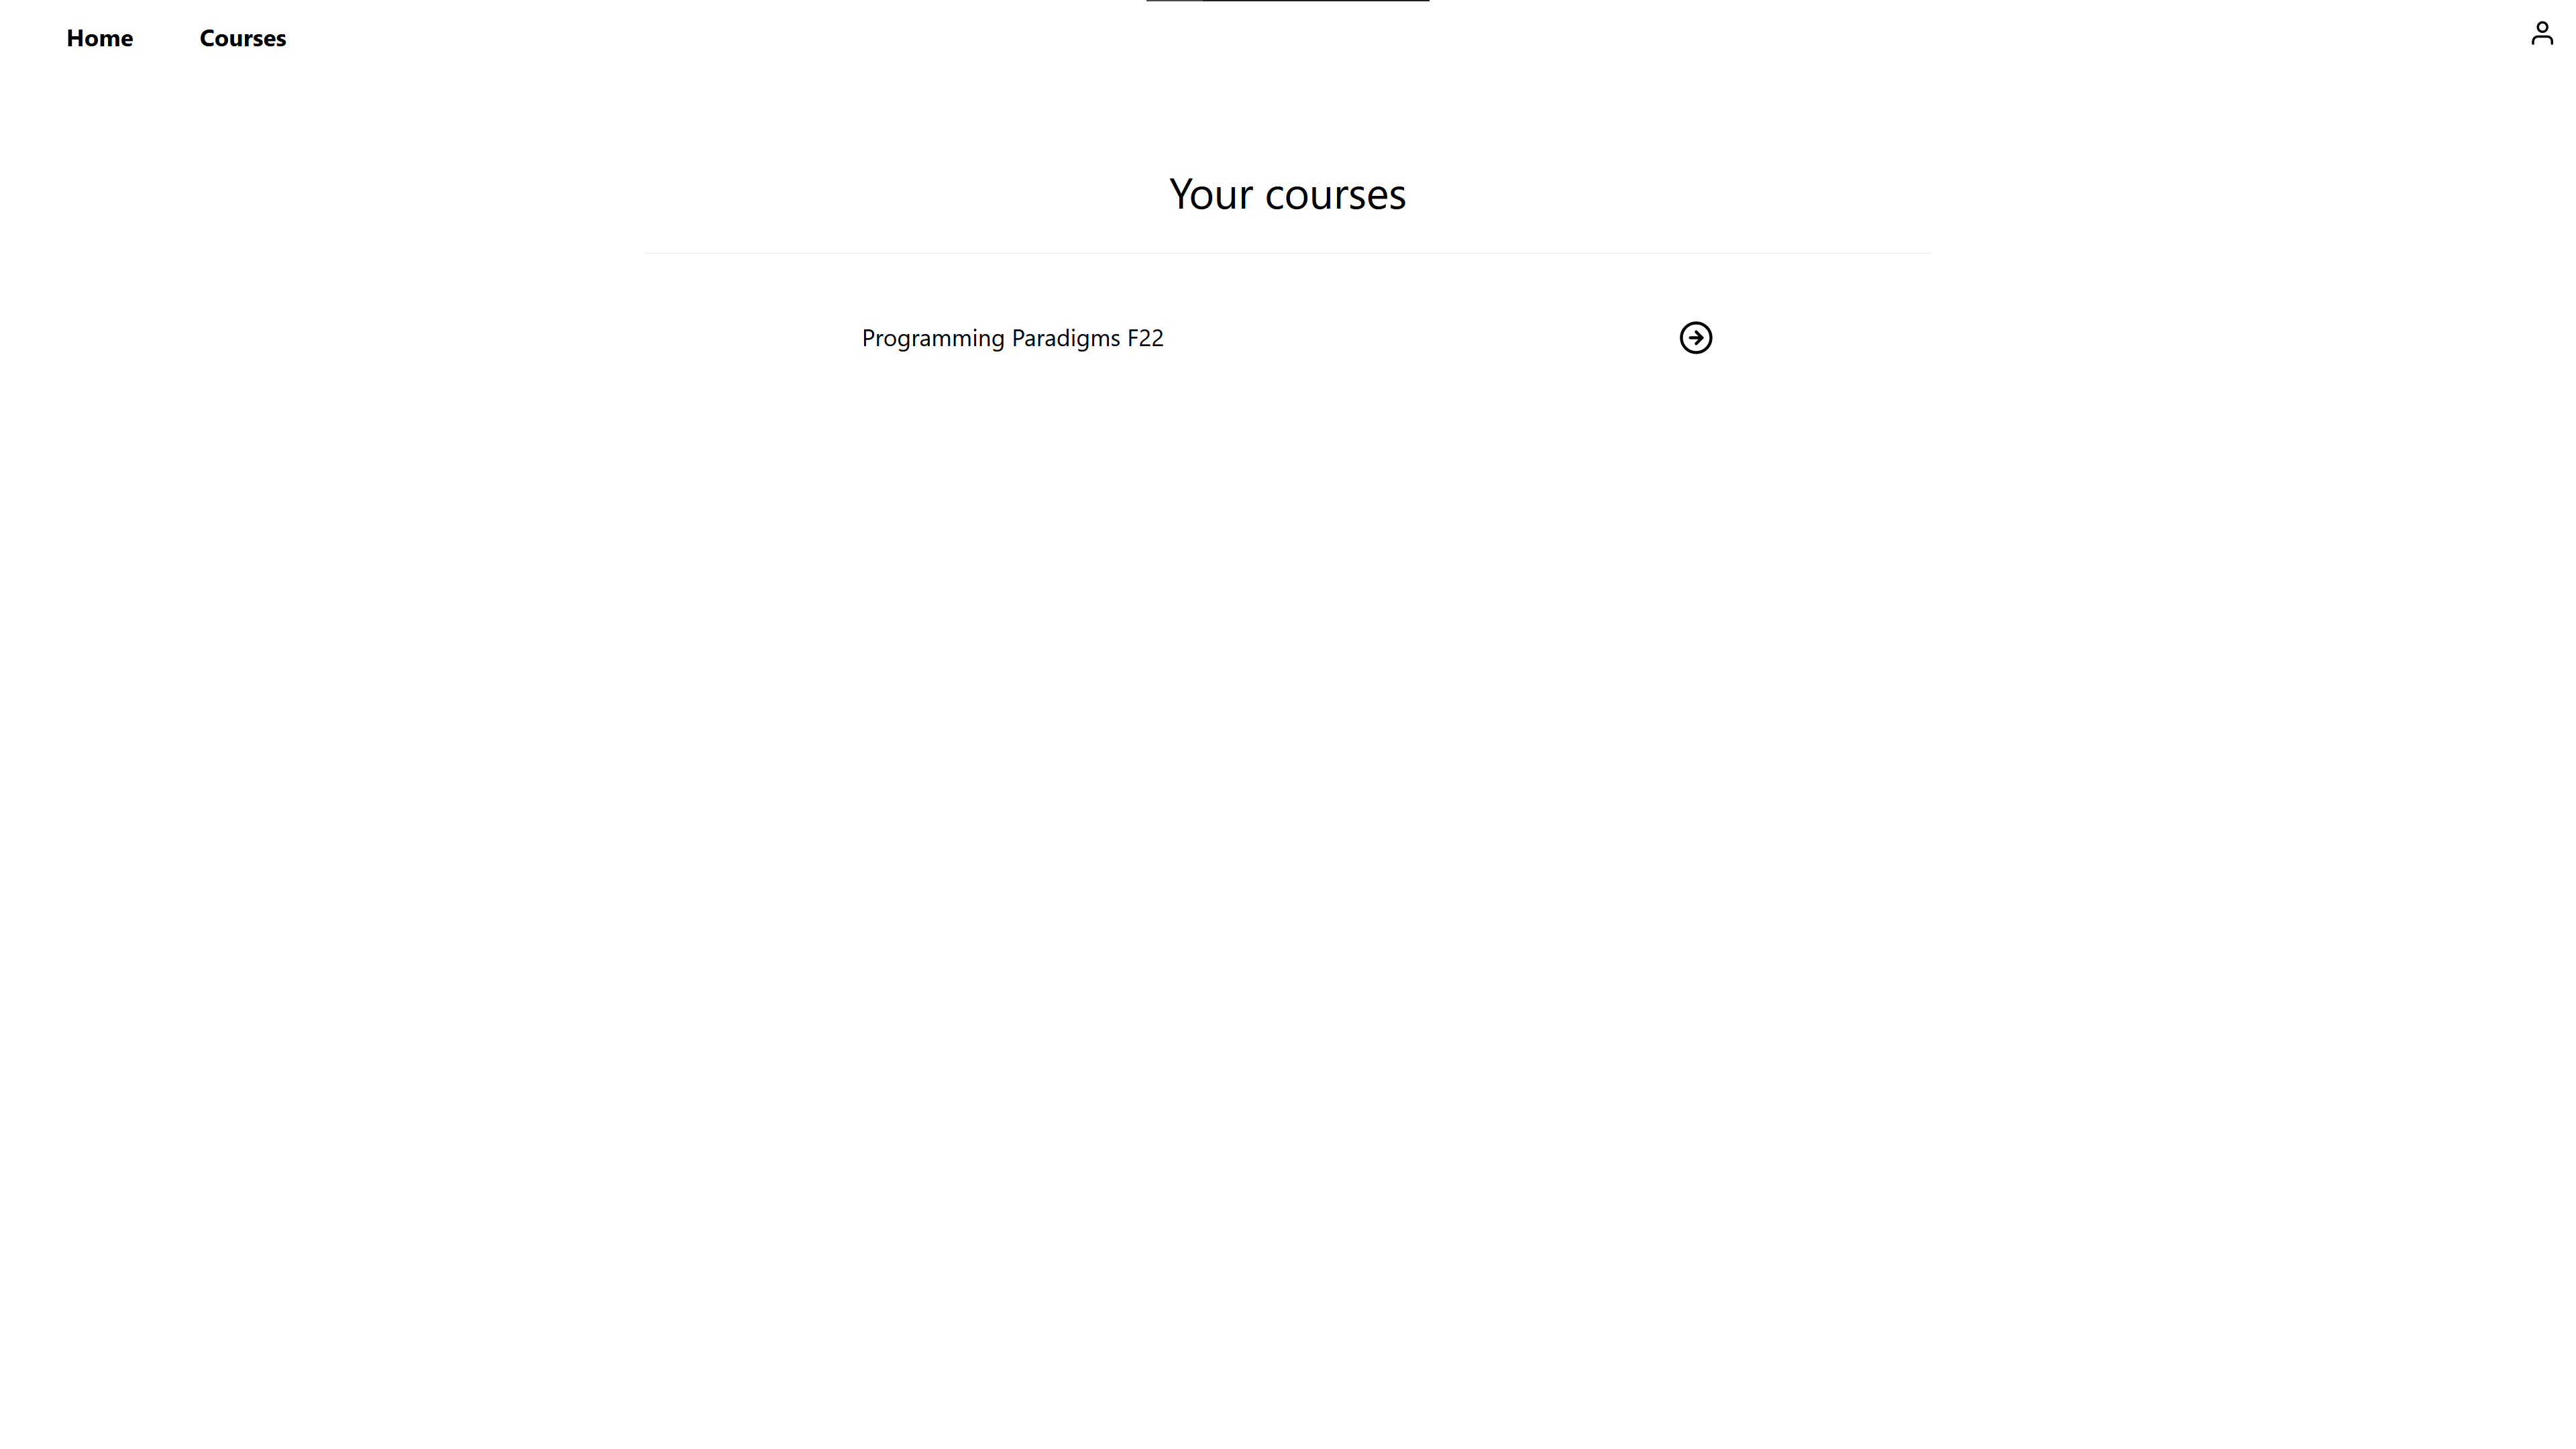
\includegraphics[scale=0.1]{syllabi.png}}
    \caption{Syllabi overview as a logged-in student}
    \label{fig:syllabi}
\end{figure}

\begin{figure}[H]
    \centering
    \frame{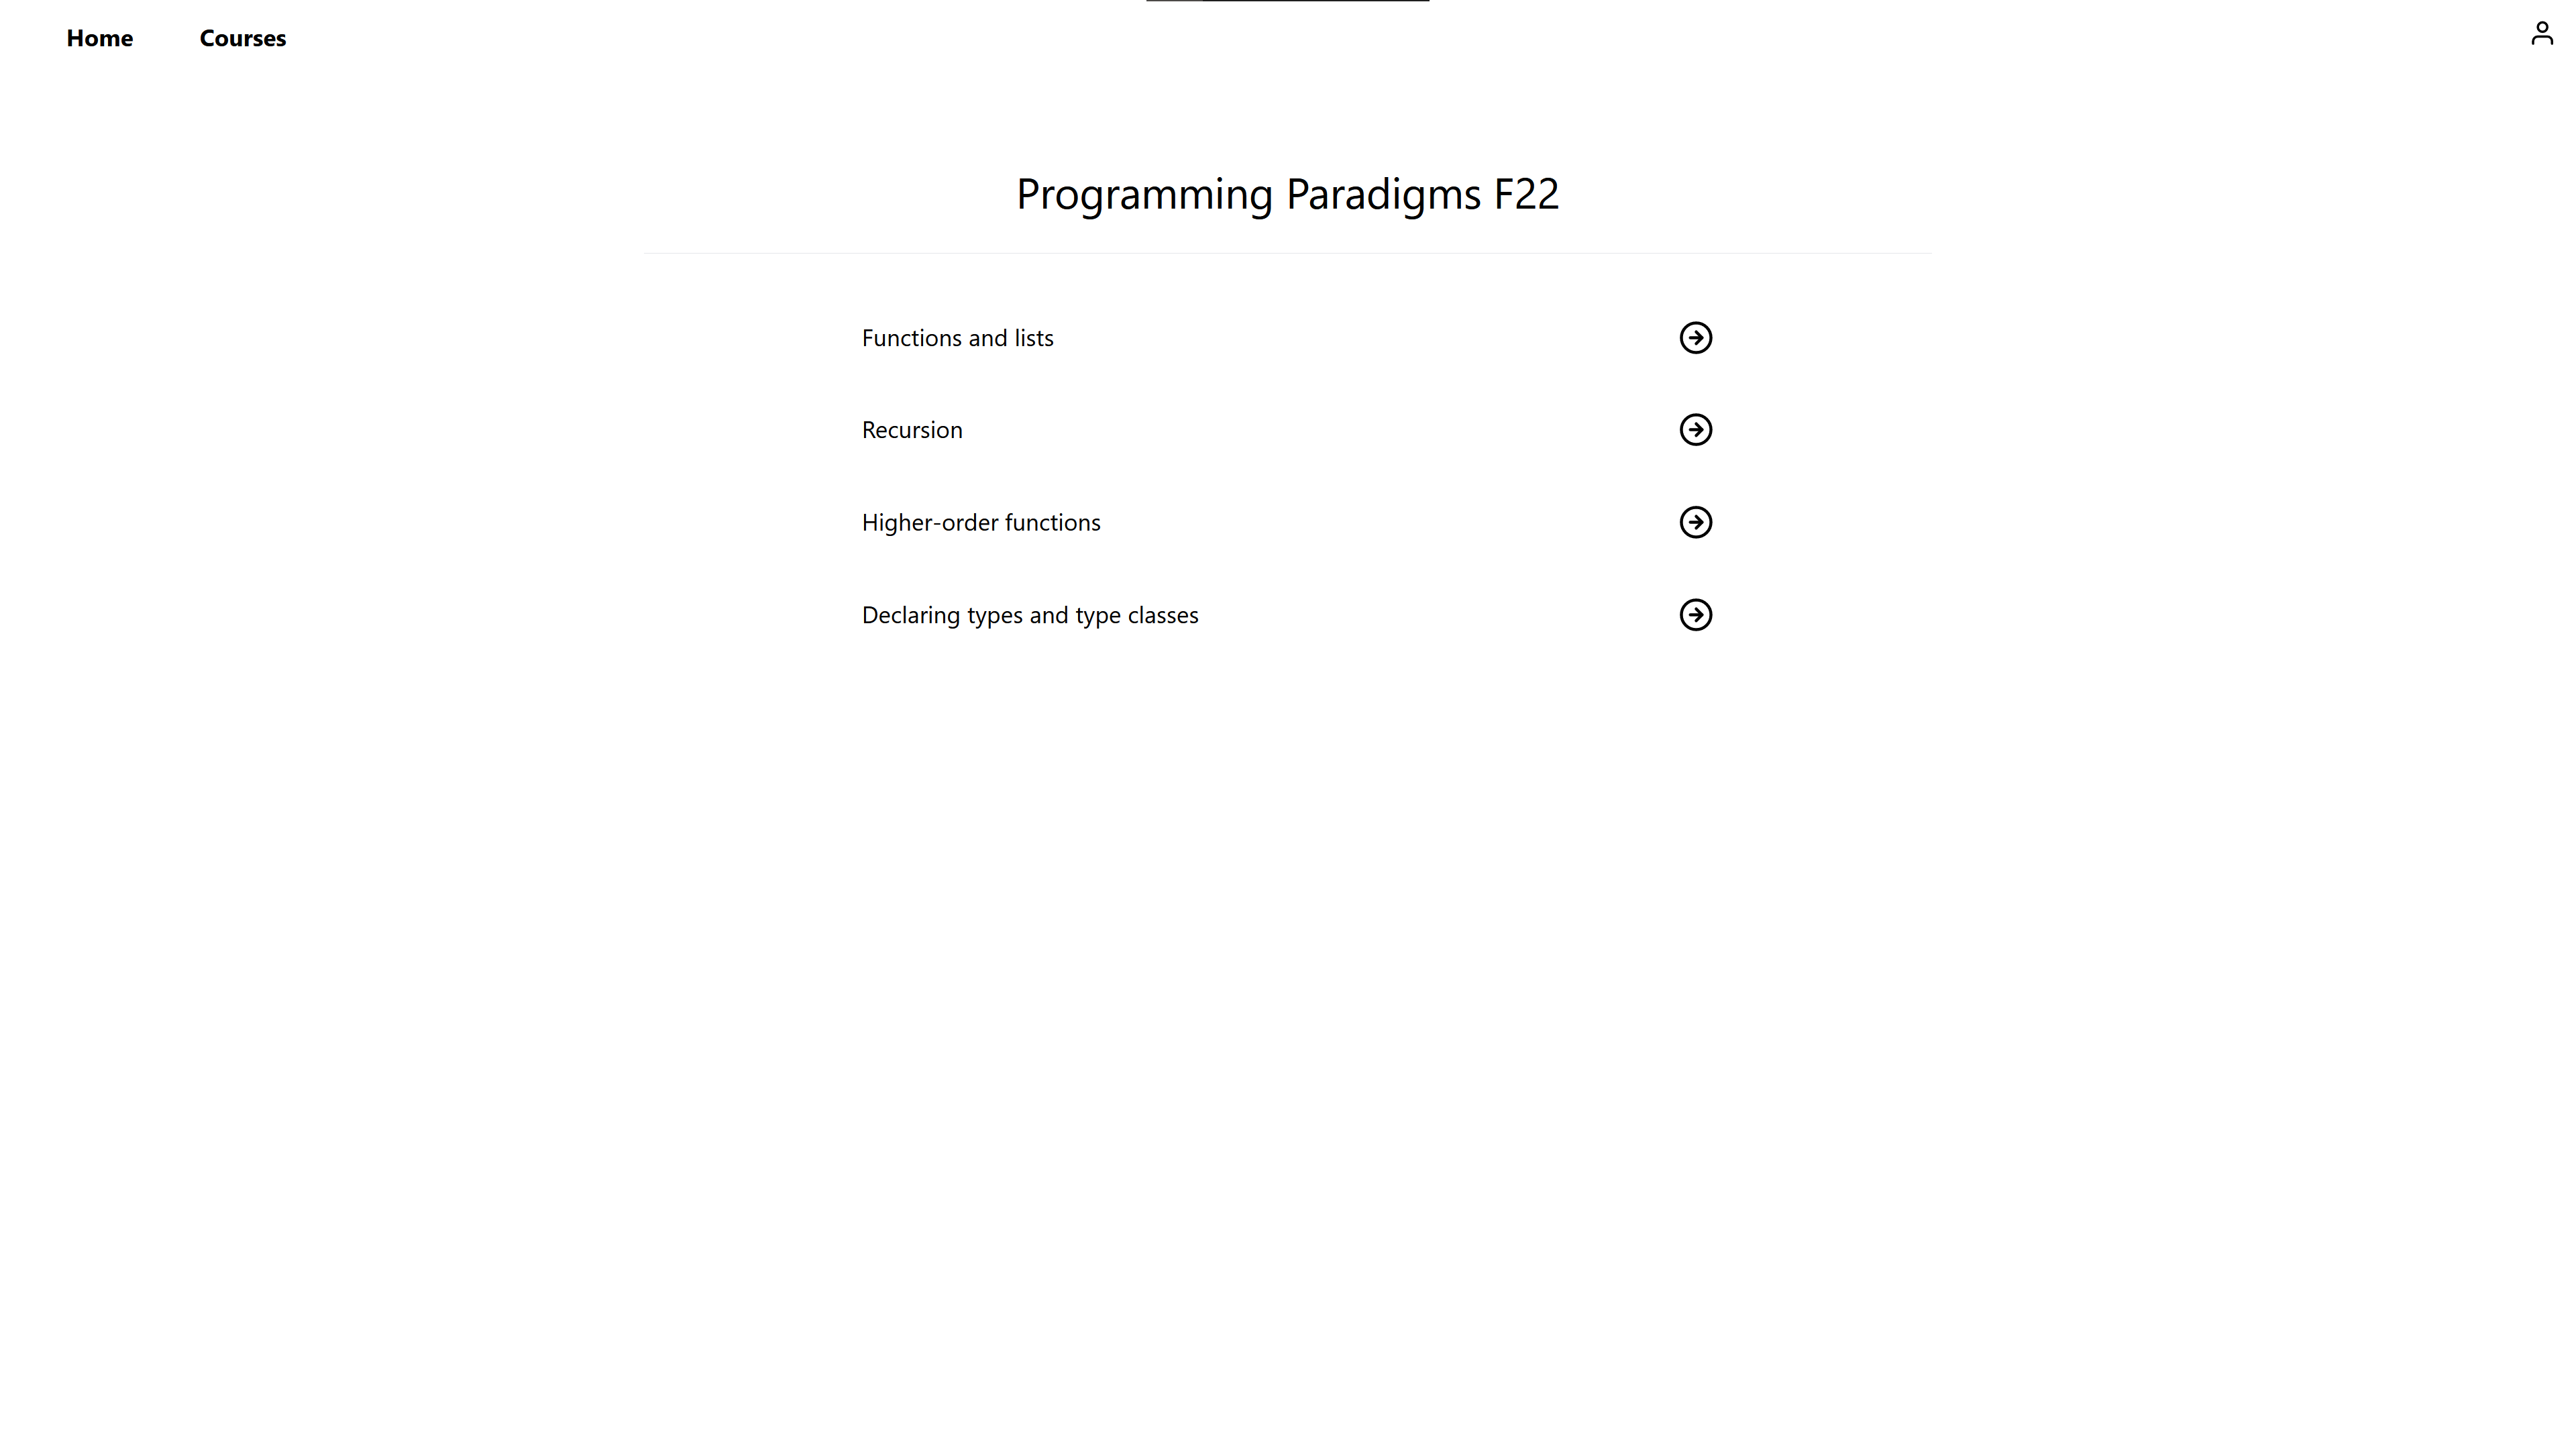
\includegraphics[scale=0.1]{problemsets.png}}
    \caption{Problem sets overview as a logged-in student}
    \label{fig:problemsets}
\end{figure}

\begin{figure}[H]
    \centering
    \frame{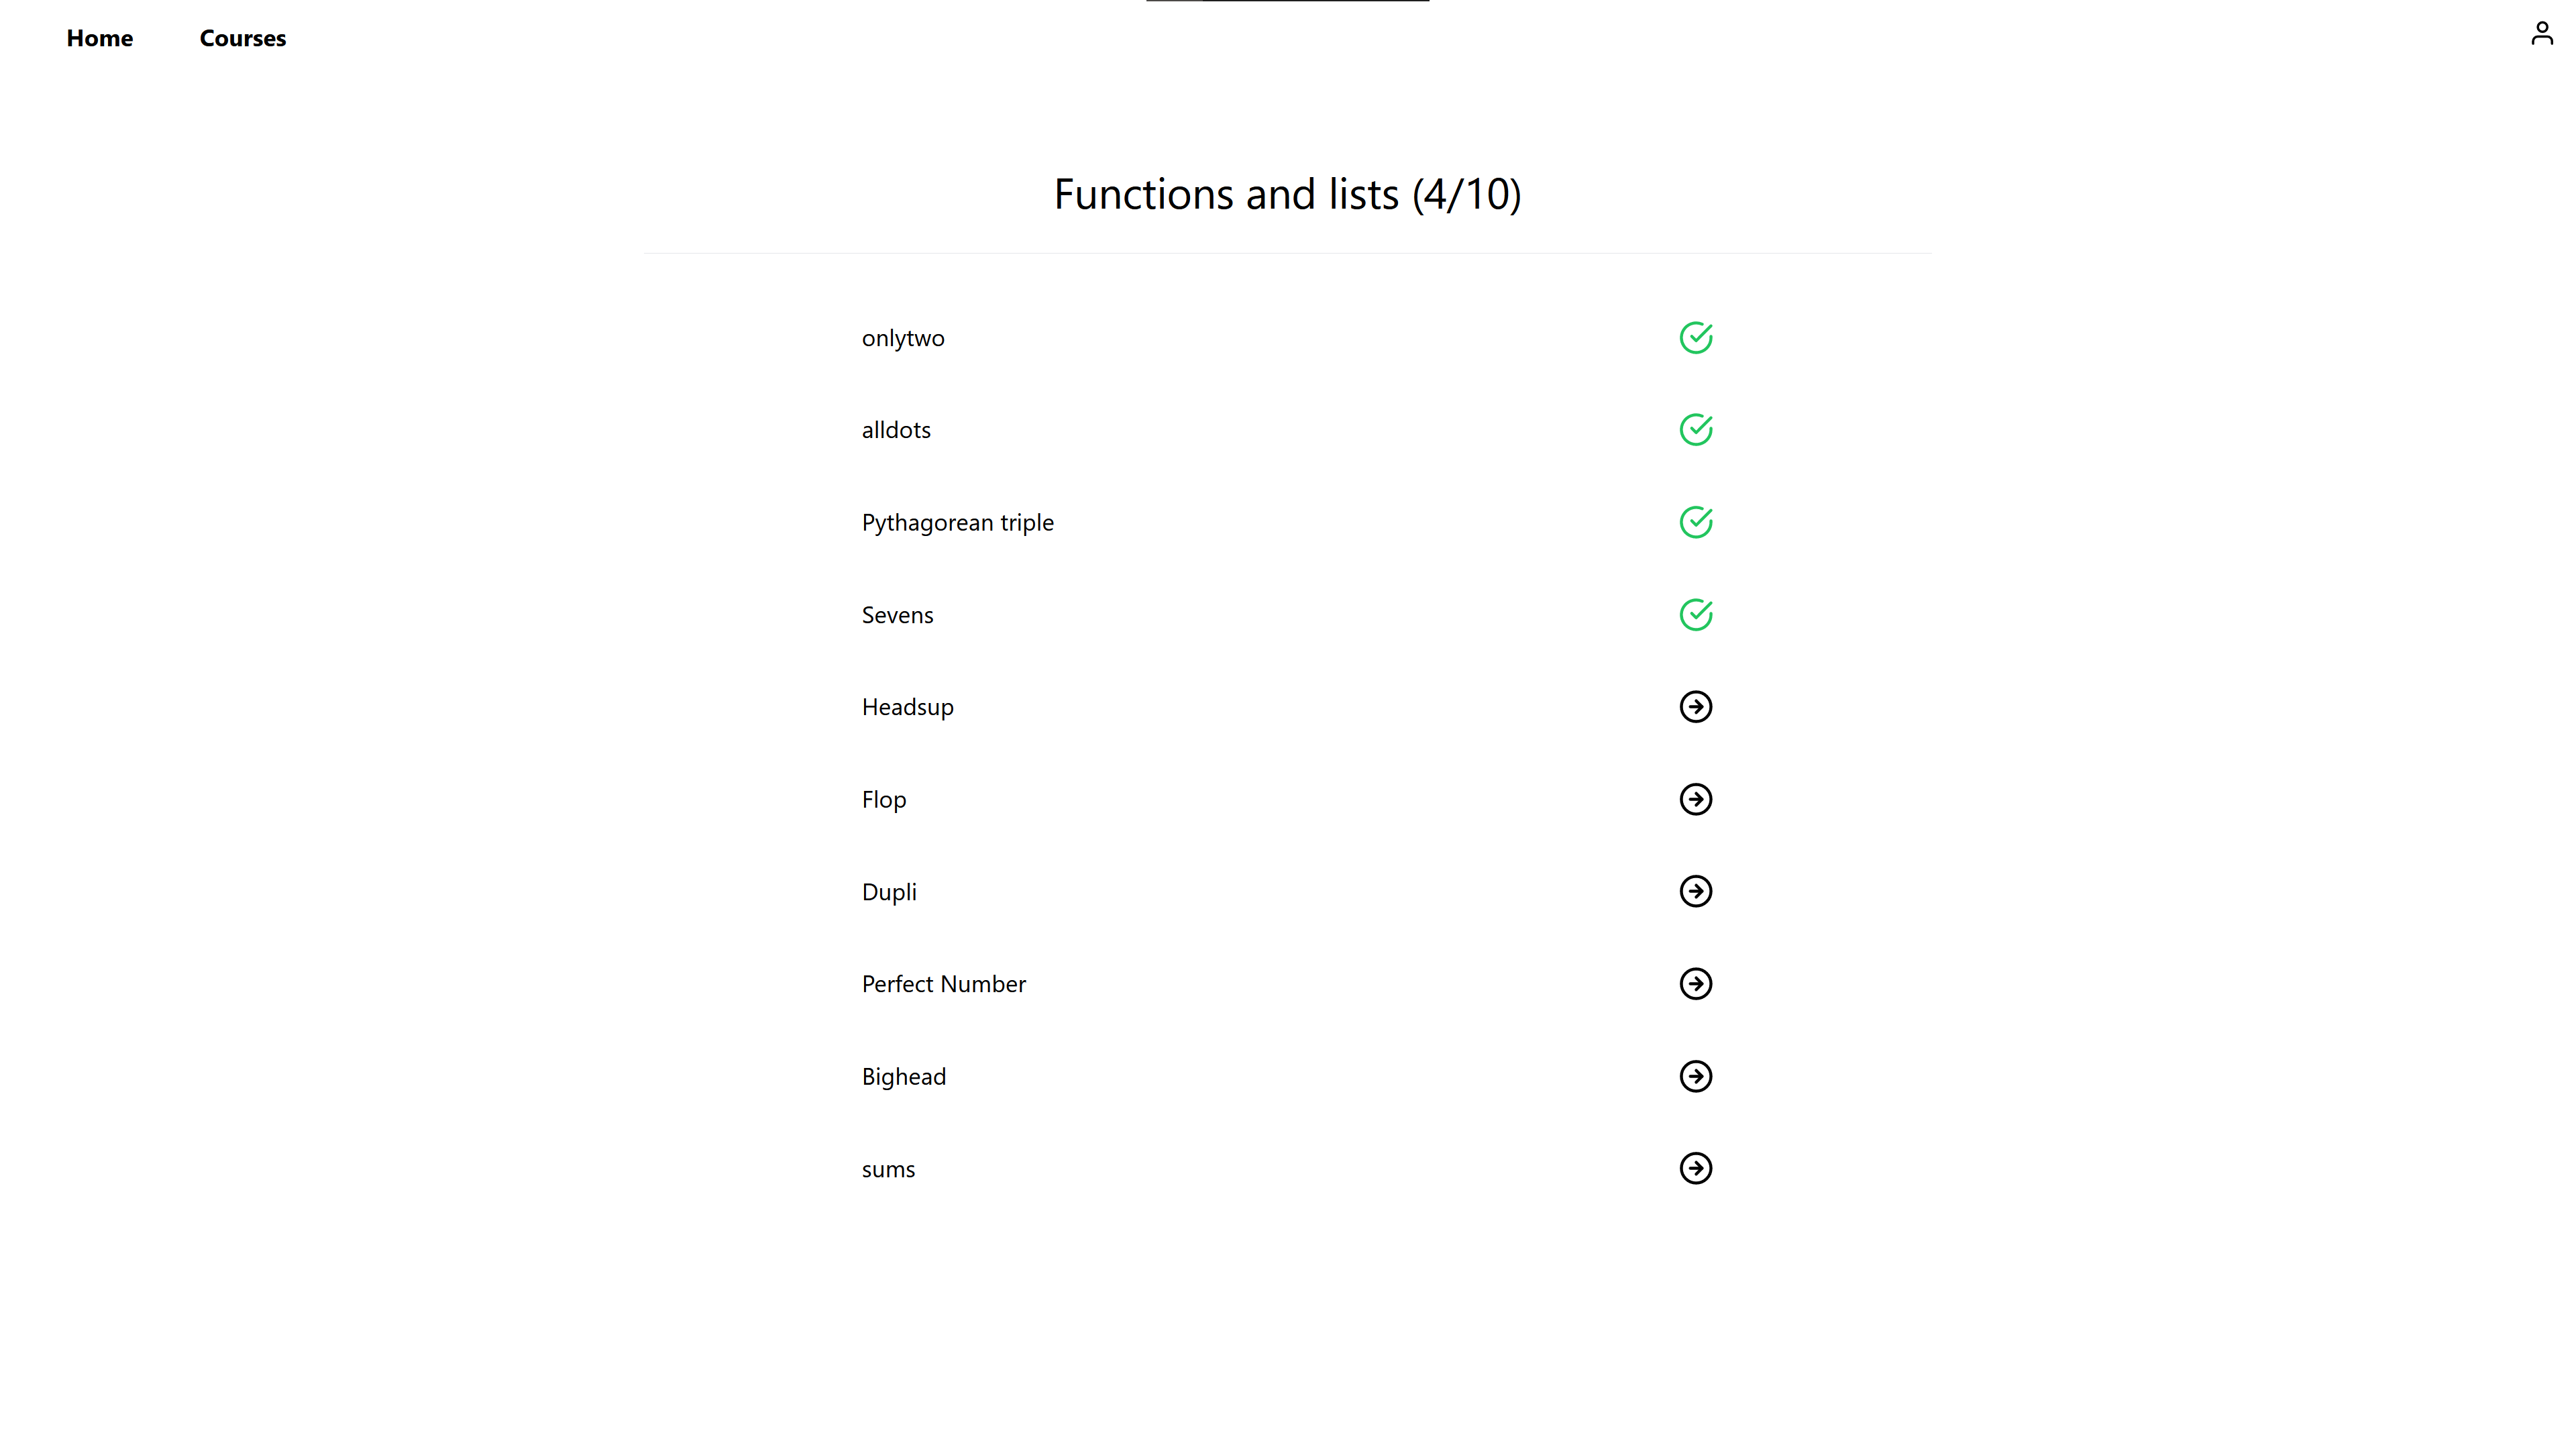
\includegraphics[scale=0.1]{exercises.png}}
    \caption{Exercise overview}
    \label{fig:exercise_overview}
\end{figure}

\begin{figure}[H]
    \centering
    \frame{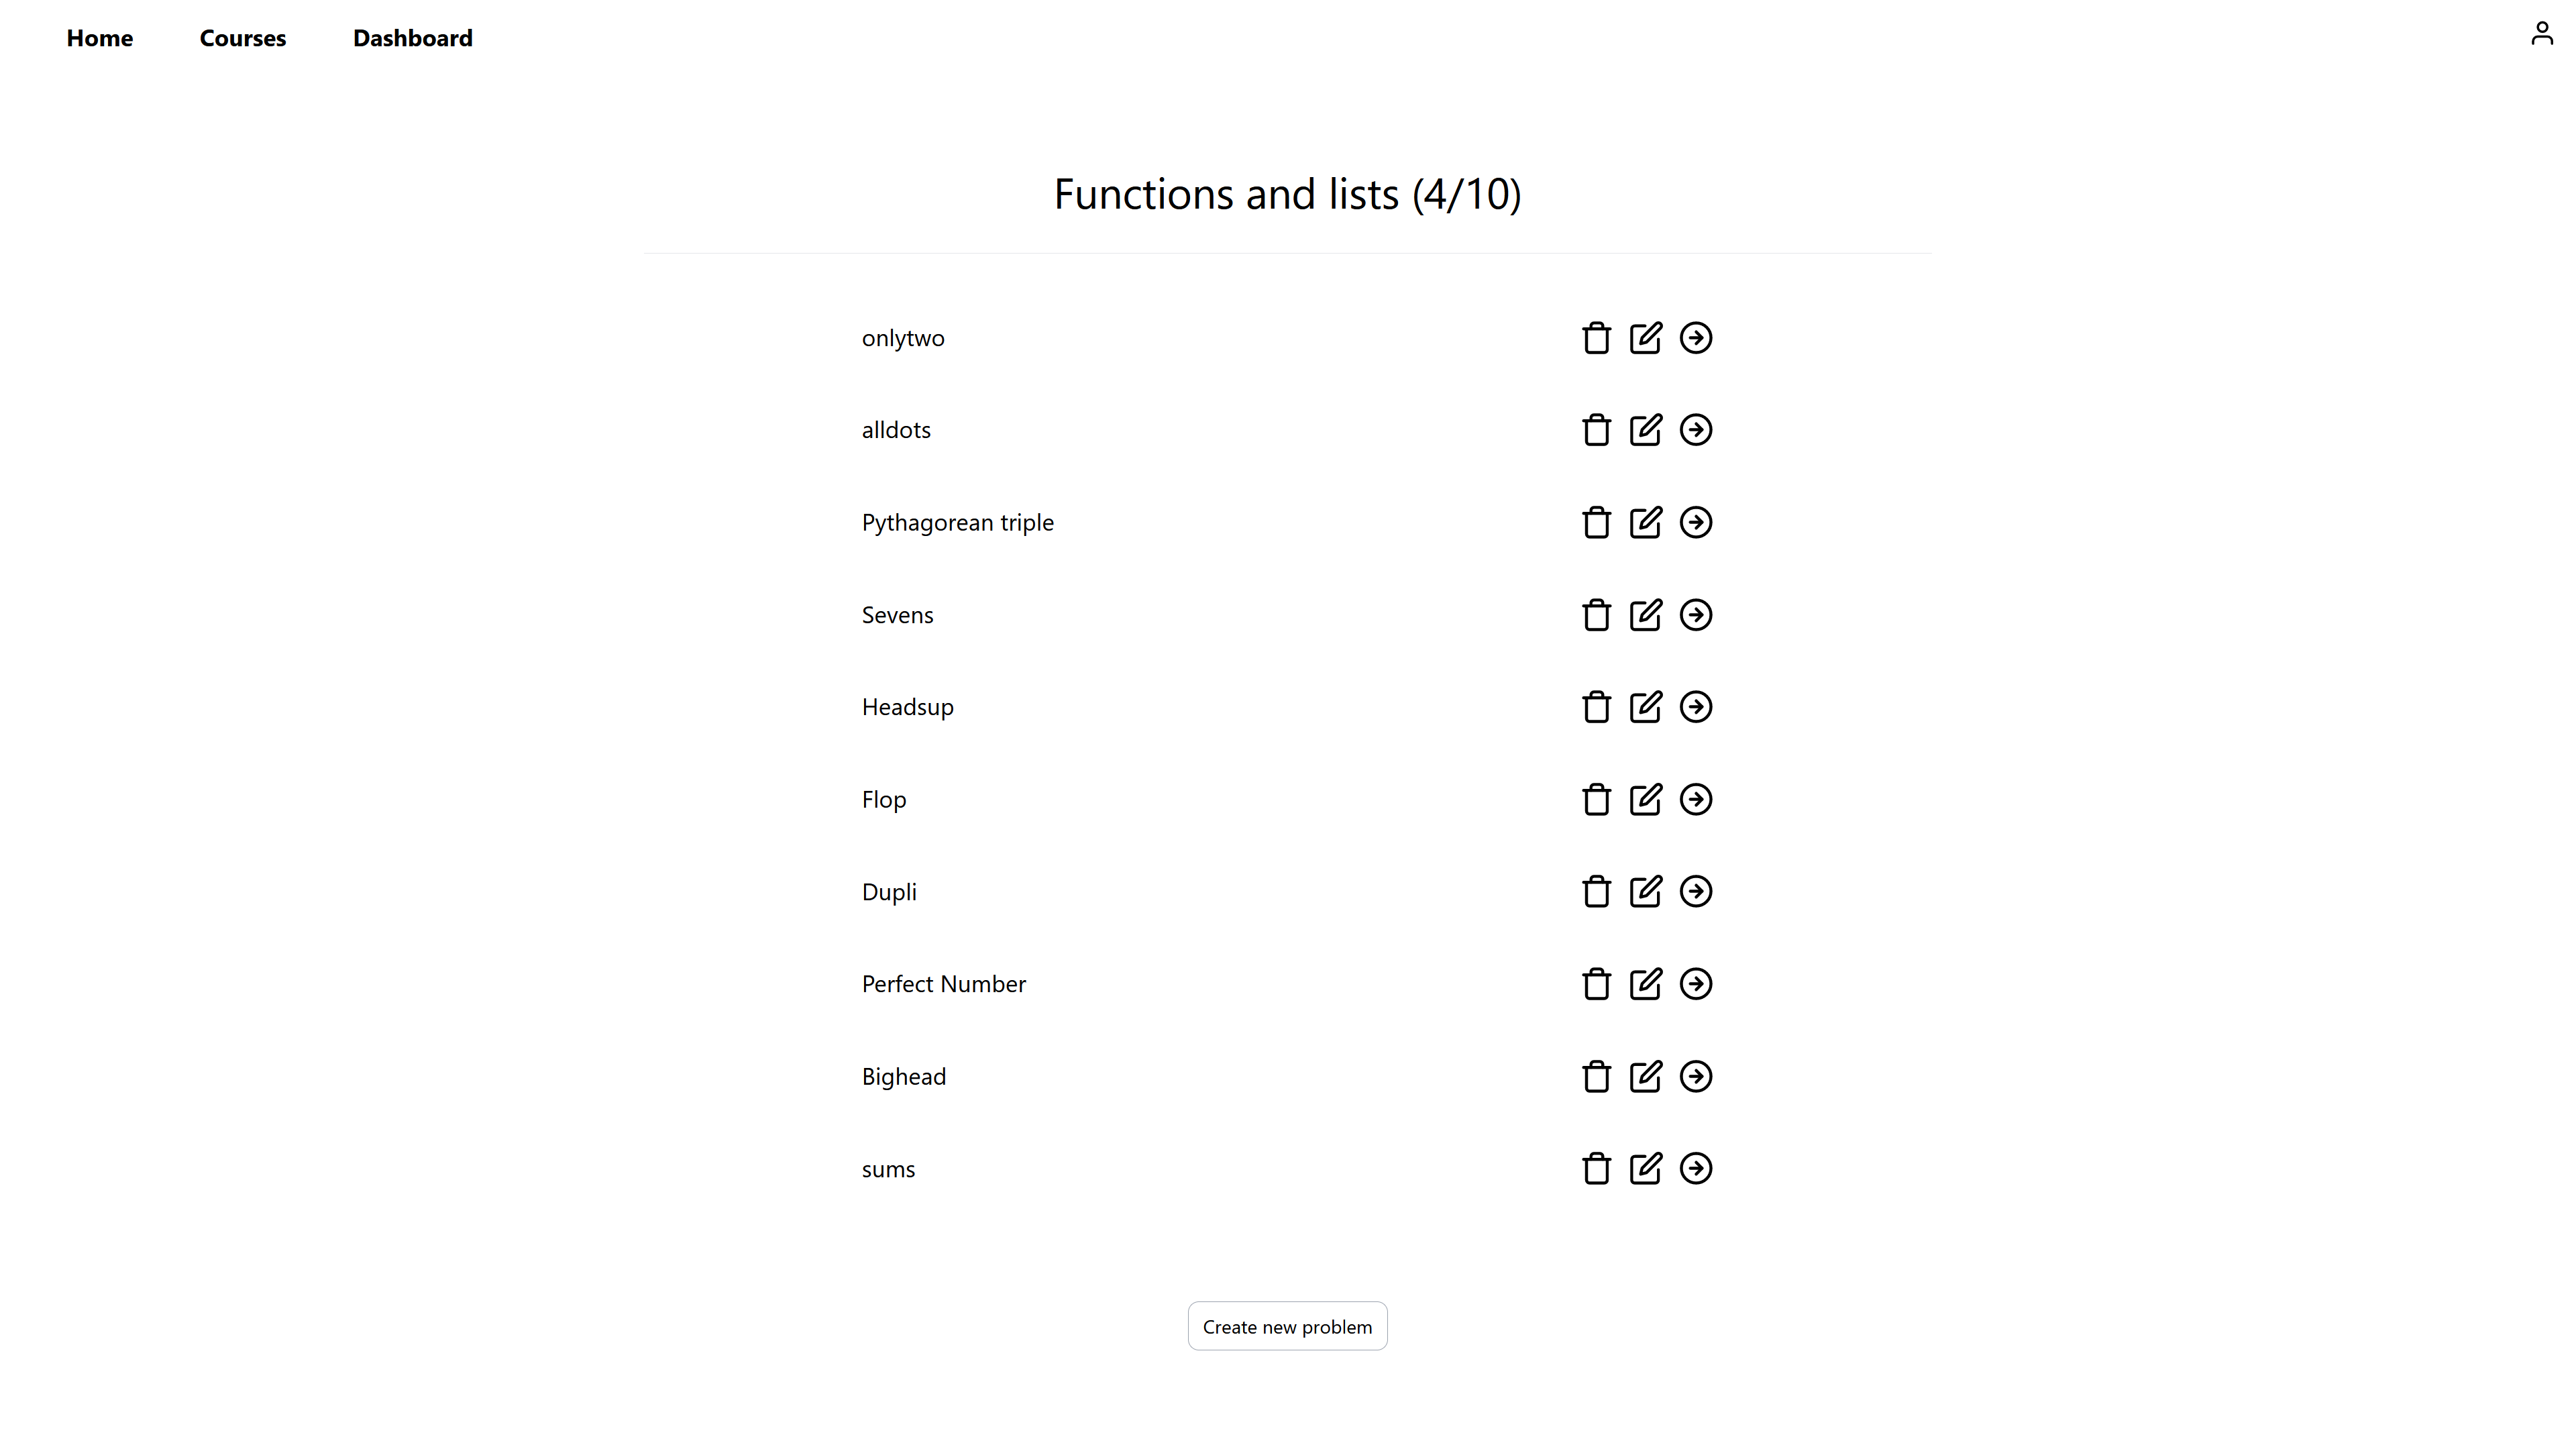
\includegraphics[scale=0.1]{problemsets_teacher_view.png}}
    \caption{Problem sets overview as a logged-in lecturer}
    \label{fig:problemsets_teacher_view}
\end{figure}

\section{Problem View and Code Editor}
When a user visits a page on our website, we fetch the code template exercise on the server in order to prevent flashing in the template after the page has loaded.
This is important because, without this, users with slow internet connections might see the template being overwritten after they have already started writing in it. That is, if you don't disable the input field entirely until the page has finished loading data. Both these approaches could lead to confusion and frustration for the user, so we decided to fetch the template before the page is rendered.

Once the UI for the page is rendered, we fetch the problem, test, and previous submissions for the user.
This allows them to see the information they need in order to solve the exercise and see their previous submissions.
The code editor on the page uses CodeMirror with extensions to support multiple programming languages.
Currently, only Haskell is supported, but it is easiy extensible to include other languages.
We have also developed a custom extension to propagate state to the parent component, which allows us to retrieve the code from the editor and send it to the backend.
In addition to allowing users to submit their code, we also fetch their previous submissions from the backend.
This allows users to revisit their previous submissions and see the date they were submitted, as well as whether they solved the exercise.
This can be useful for users who want to track their progress or review their previous work.

% - Session extension så vi kan handle auth igennem session. Tilføjet rolle til session så vi kan håndtere permissions på forskellige sider.
% - Sidernes indhold muteres baseret på brugerens rolle. Håndtere også hvis du ikke er logget ind.
% - TRPC til at hendte data fra databasen. Sker via API kald, således at eksempelvis SQL kald ikke sker direkte fra frontenden.
% - Solve problem siden. Henter templates når du loader siden. Henter template før UI bliver renderet. Når ui render henter vi problem, test og tidligere submissions.
% - Code editor. Codemirror med custom extension.

\section{Client-Server Interaction}
When a lecturer creates a new exercise, a modal prompts them to enter details about the exercise.
These details include the name of the exercise, instructions for the student, an optional code template to help the student get started, as well as test code.
This data is sent to the database where it is stored.
When a student opens an exercise, the data is then fetched from the database.
This is done by the client sending a request to the Next.js backend, which queries the database and returns both exercise and test data.

\begin{figure}[H]
    \centering
    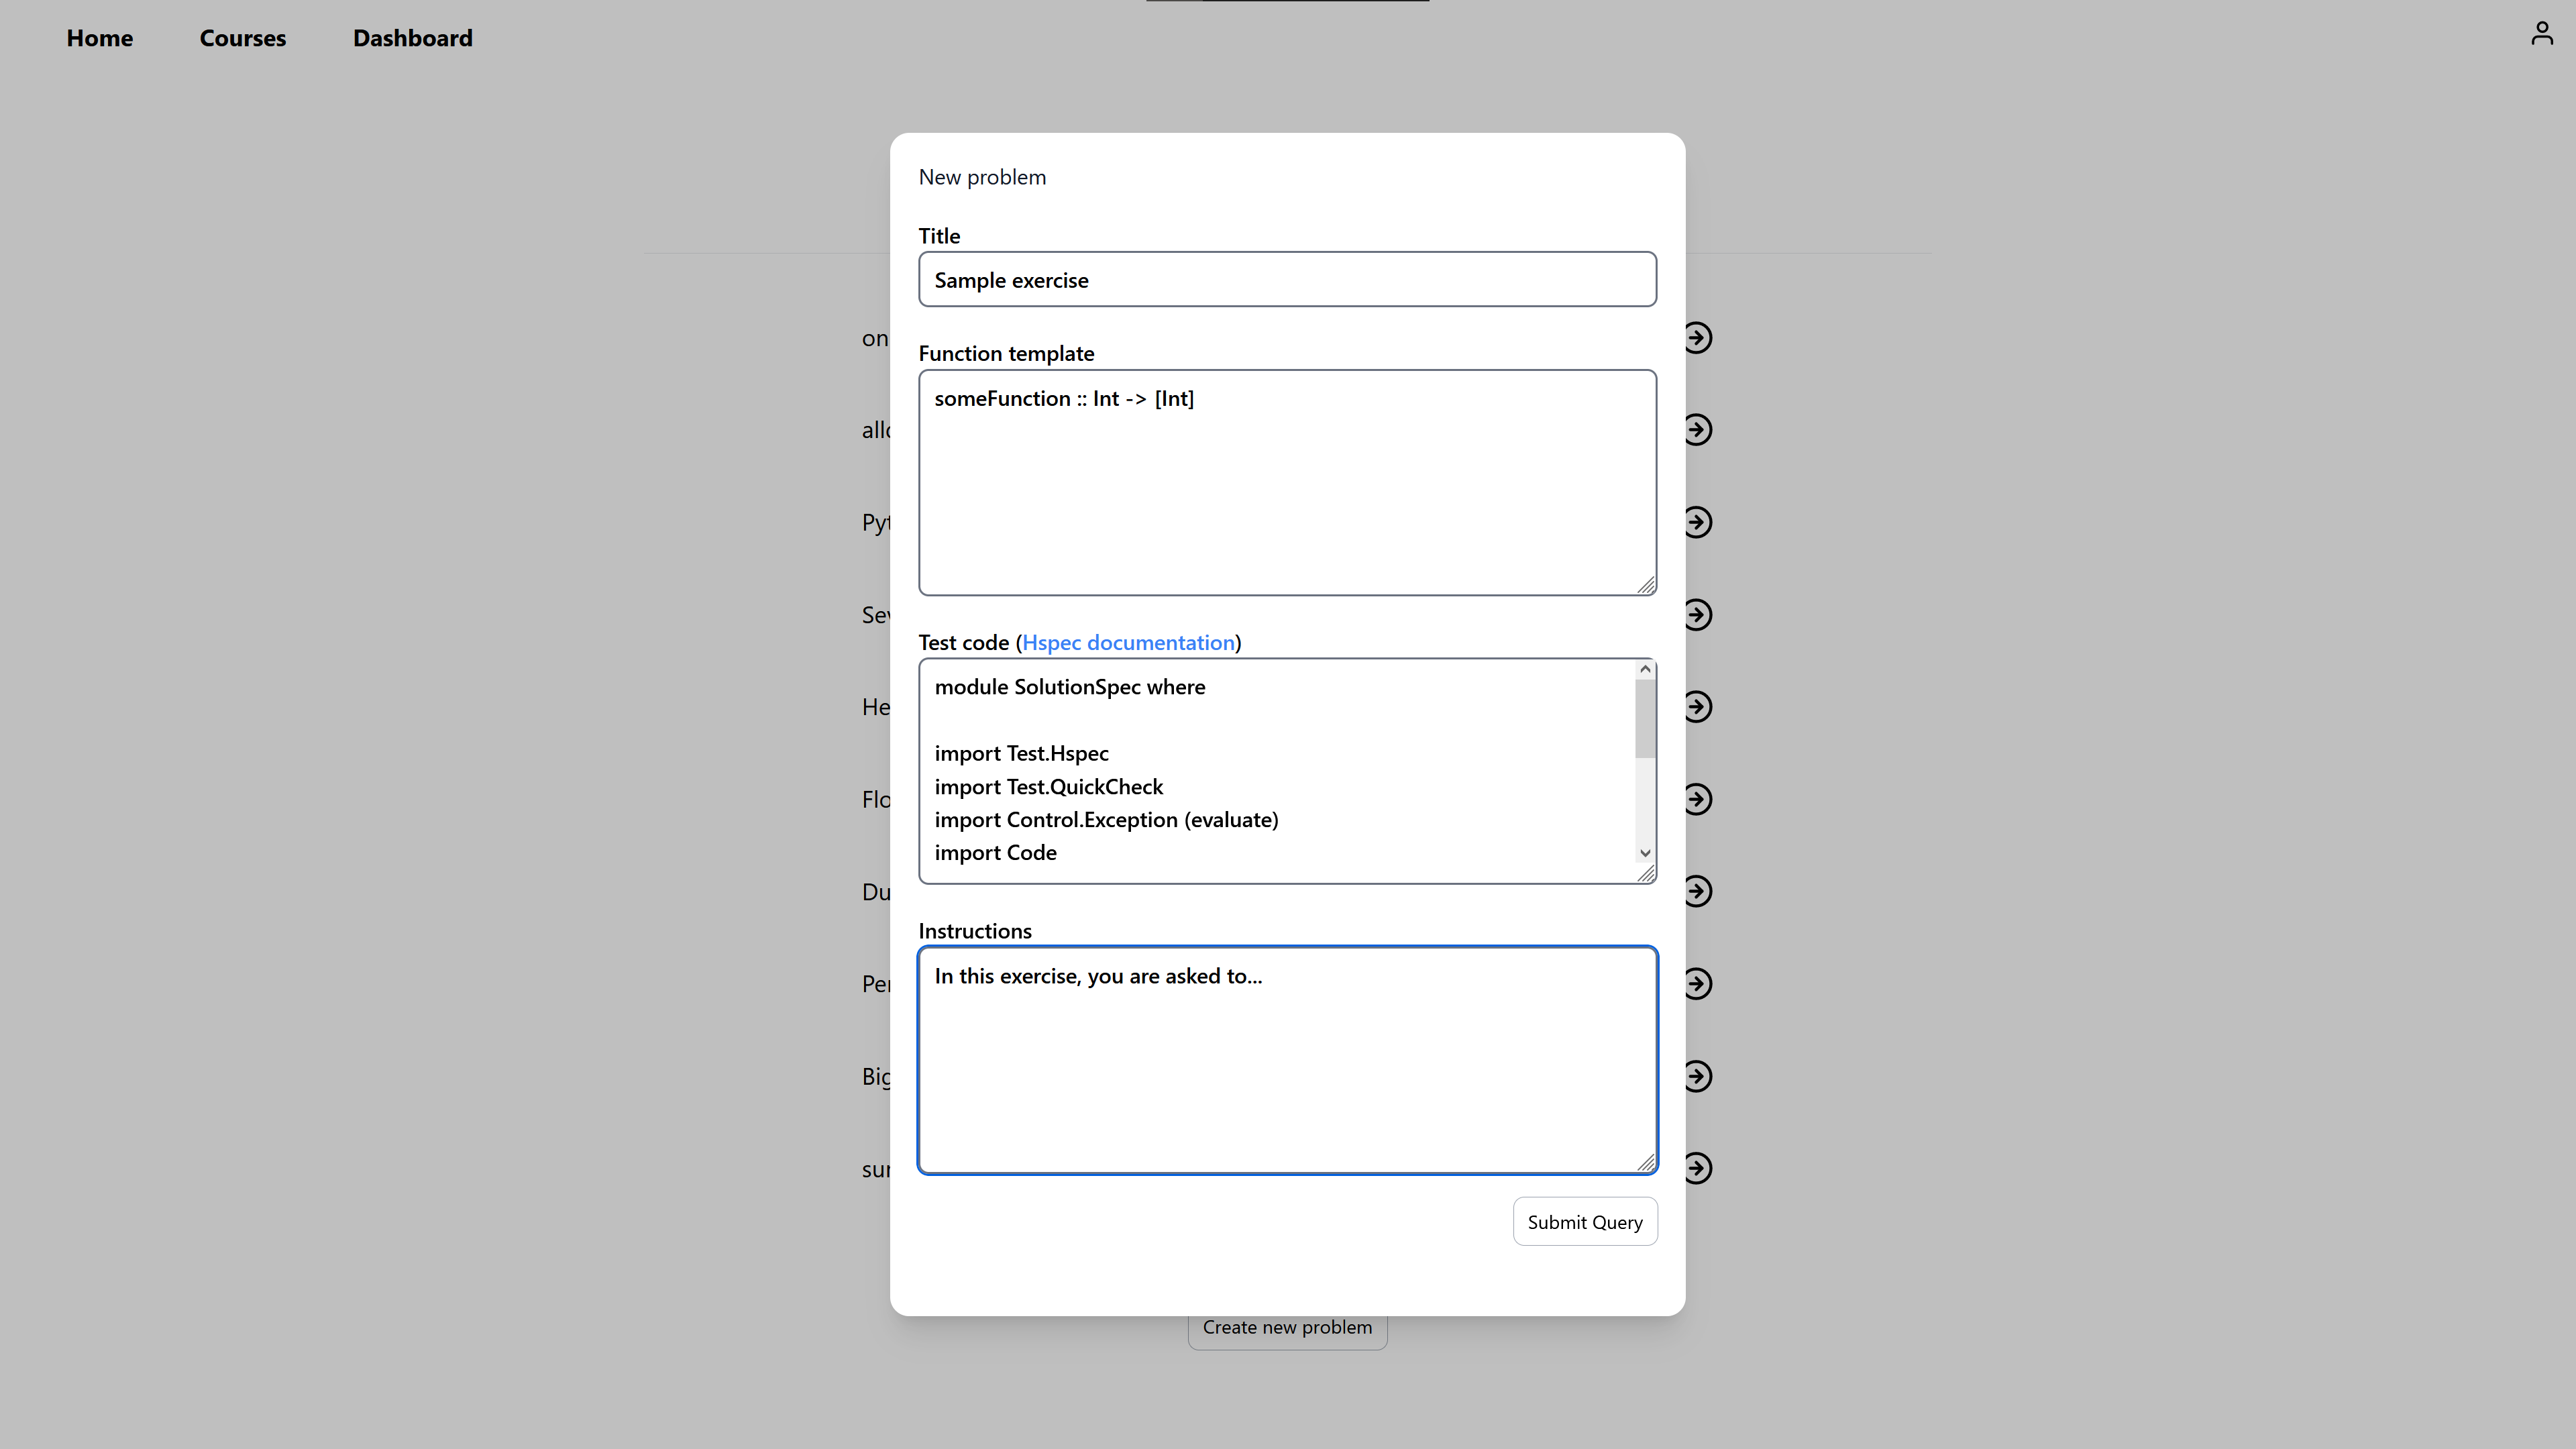
\includegraphics[scale=0.1]{create_exercise.png}
    \caption{Creating a new exercise as a lecturer}
    \label{fig:create_exercise}
\end{figure}

In the interest of reducing the number of database queries, the result of this request is cached on the client.
The client will eagerly request new data to stay up to date with instructions or test code updates.
We deemed that this short cache storage time is useful for when lecturers update test code during an exercise session.
This way, all students have the latest test code shortly after the update while still minimizing unnecessary queries.

When a user submits their exercise solution attempt, a mutation is sent to the Next.js backend.
In this request, the necessary code and test code is included.
However, we want to eventually display the test code to the user so they may gain a better understanding of the solution requirements, although this will not be done in this iteration of the project.
\todo{foler ikke vi skal includere det hvis vi ikke gor det. Saa er det future works, ikke i dette afsnit}
To handle this mutation, the Next.js server requests the Test Runner to process the given solution and test code.
This process is described in chapter \ref{chap:TestRunner}.
The response of this request to the Test Runner is validated and stored as a submission in the database.
This allows users and lecturers to access previous submissions, which includes code and a value indicating whether the submission satisfied the exercise tests.
Lastly, the result is sent to the client and displayed on the page.

\begin{figure}[H]
	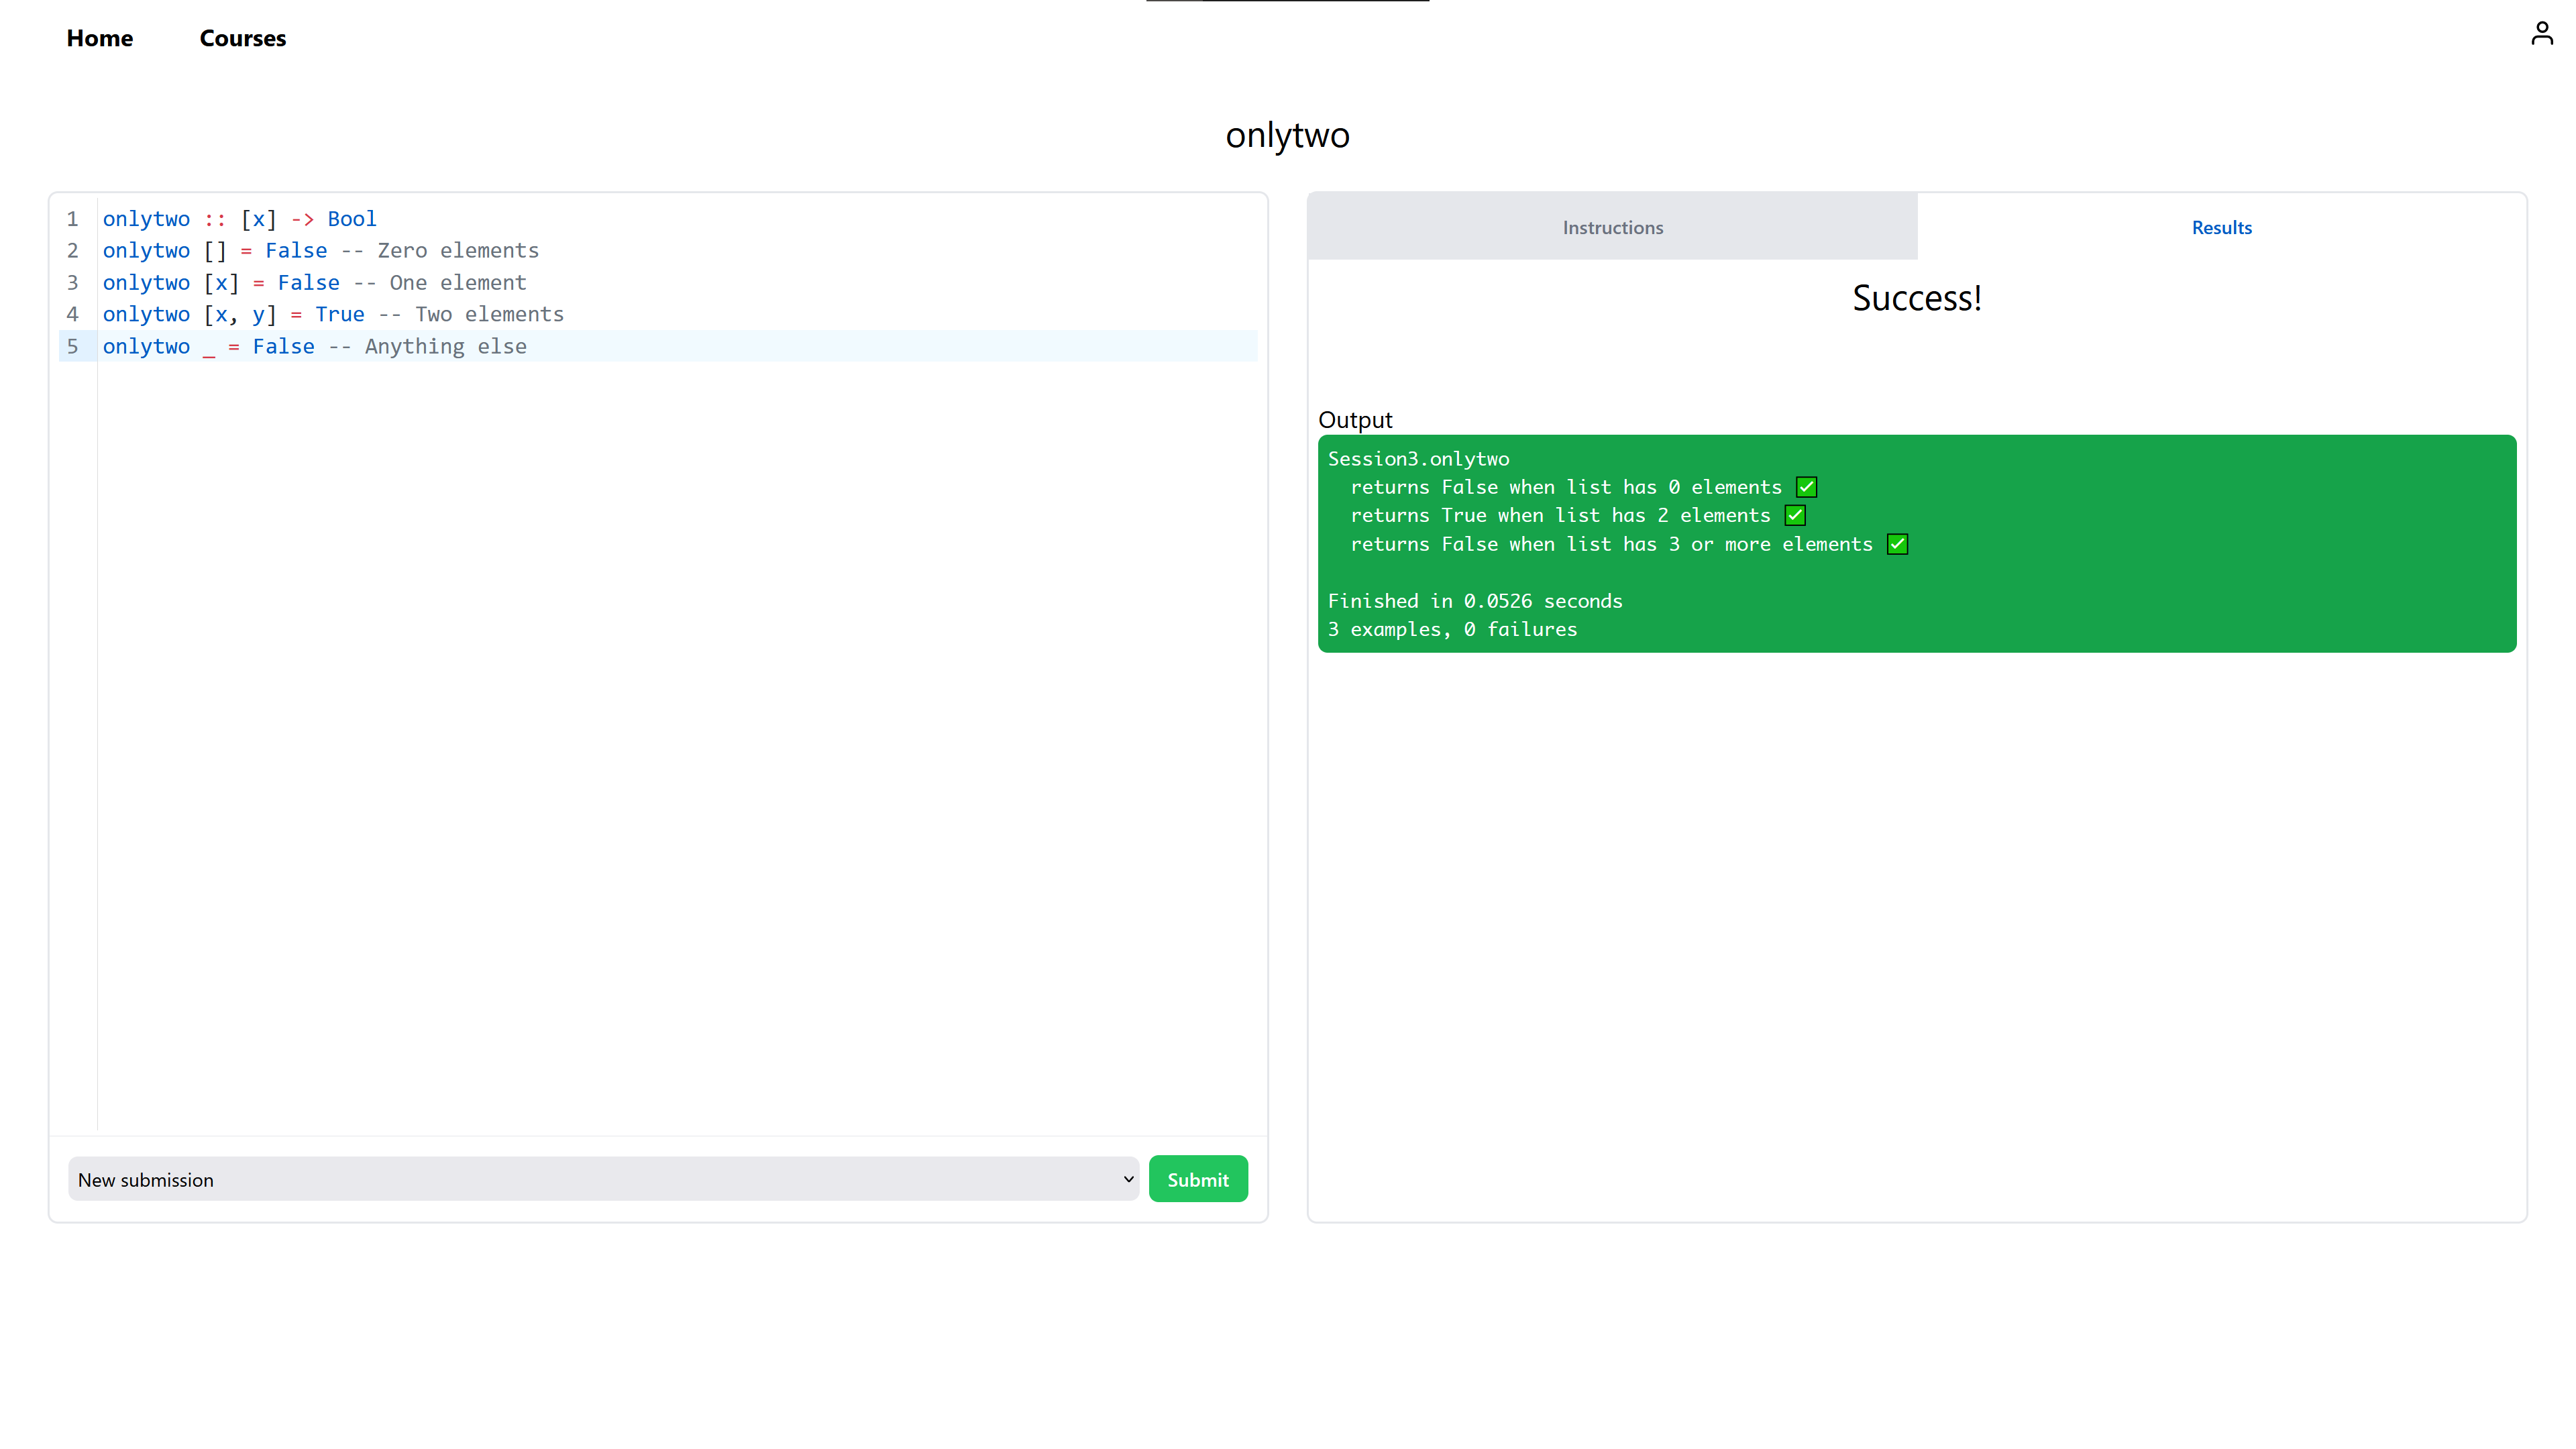
\includegraphics[scale=0.1]{exercise_success.png}
	\centering
	\caption{An example of a successful exercise submission}
	\label{fig:exercise_success}
\end{figure}

\begin{figure}[H]
	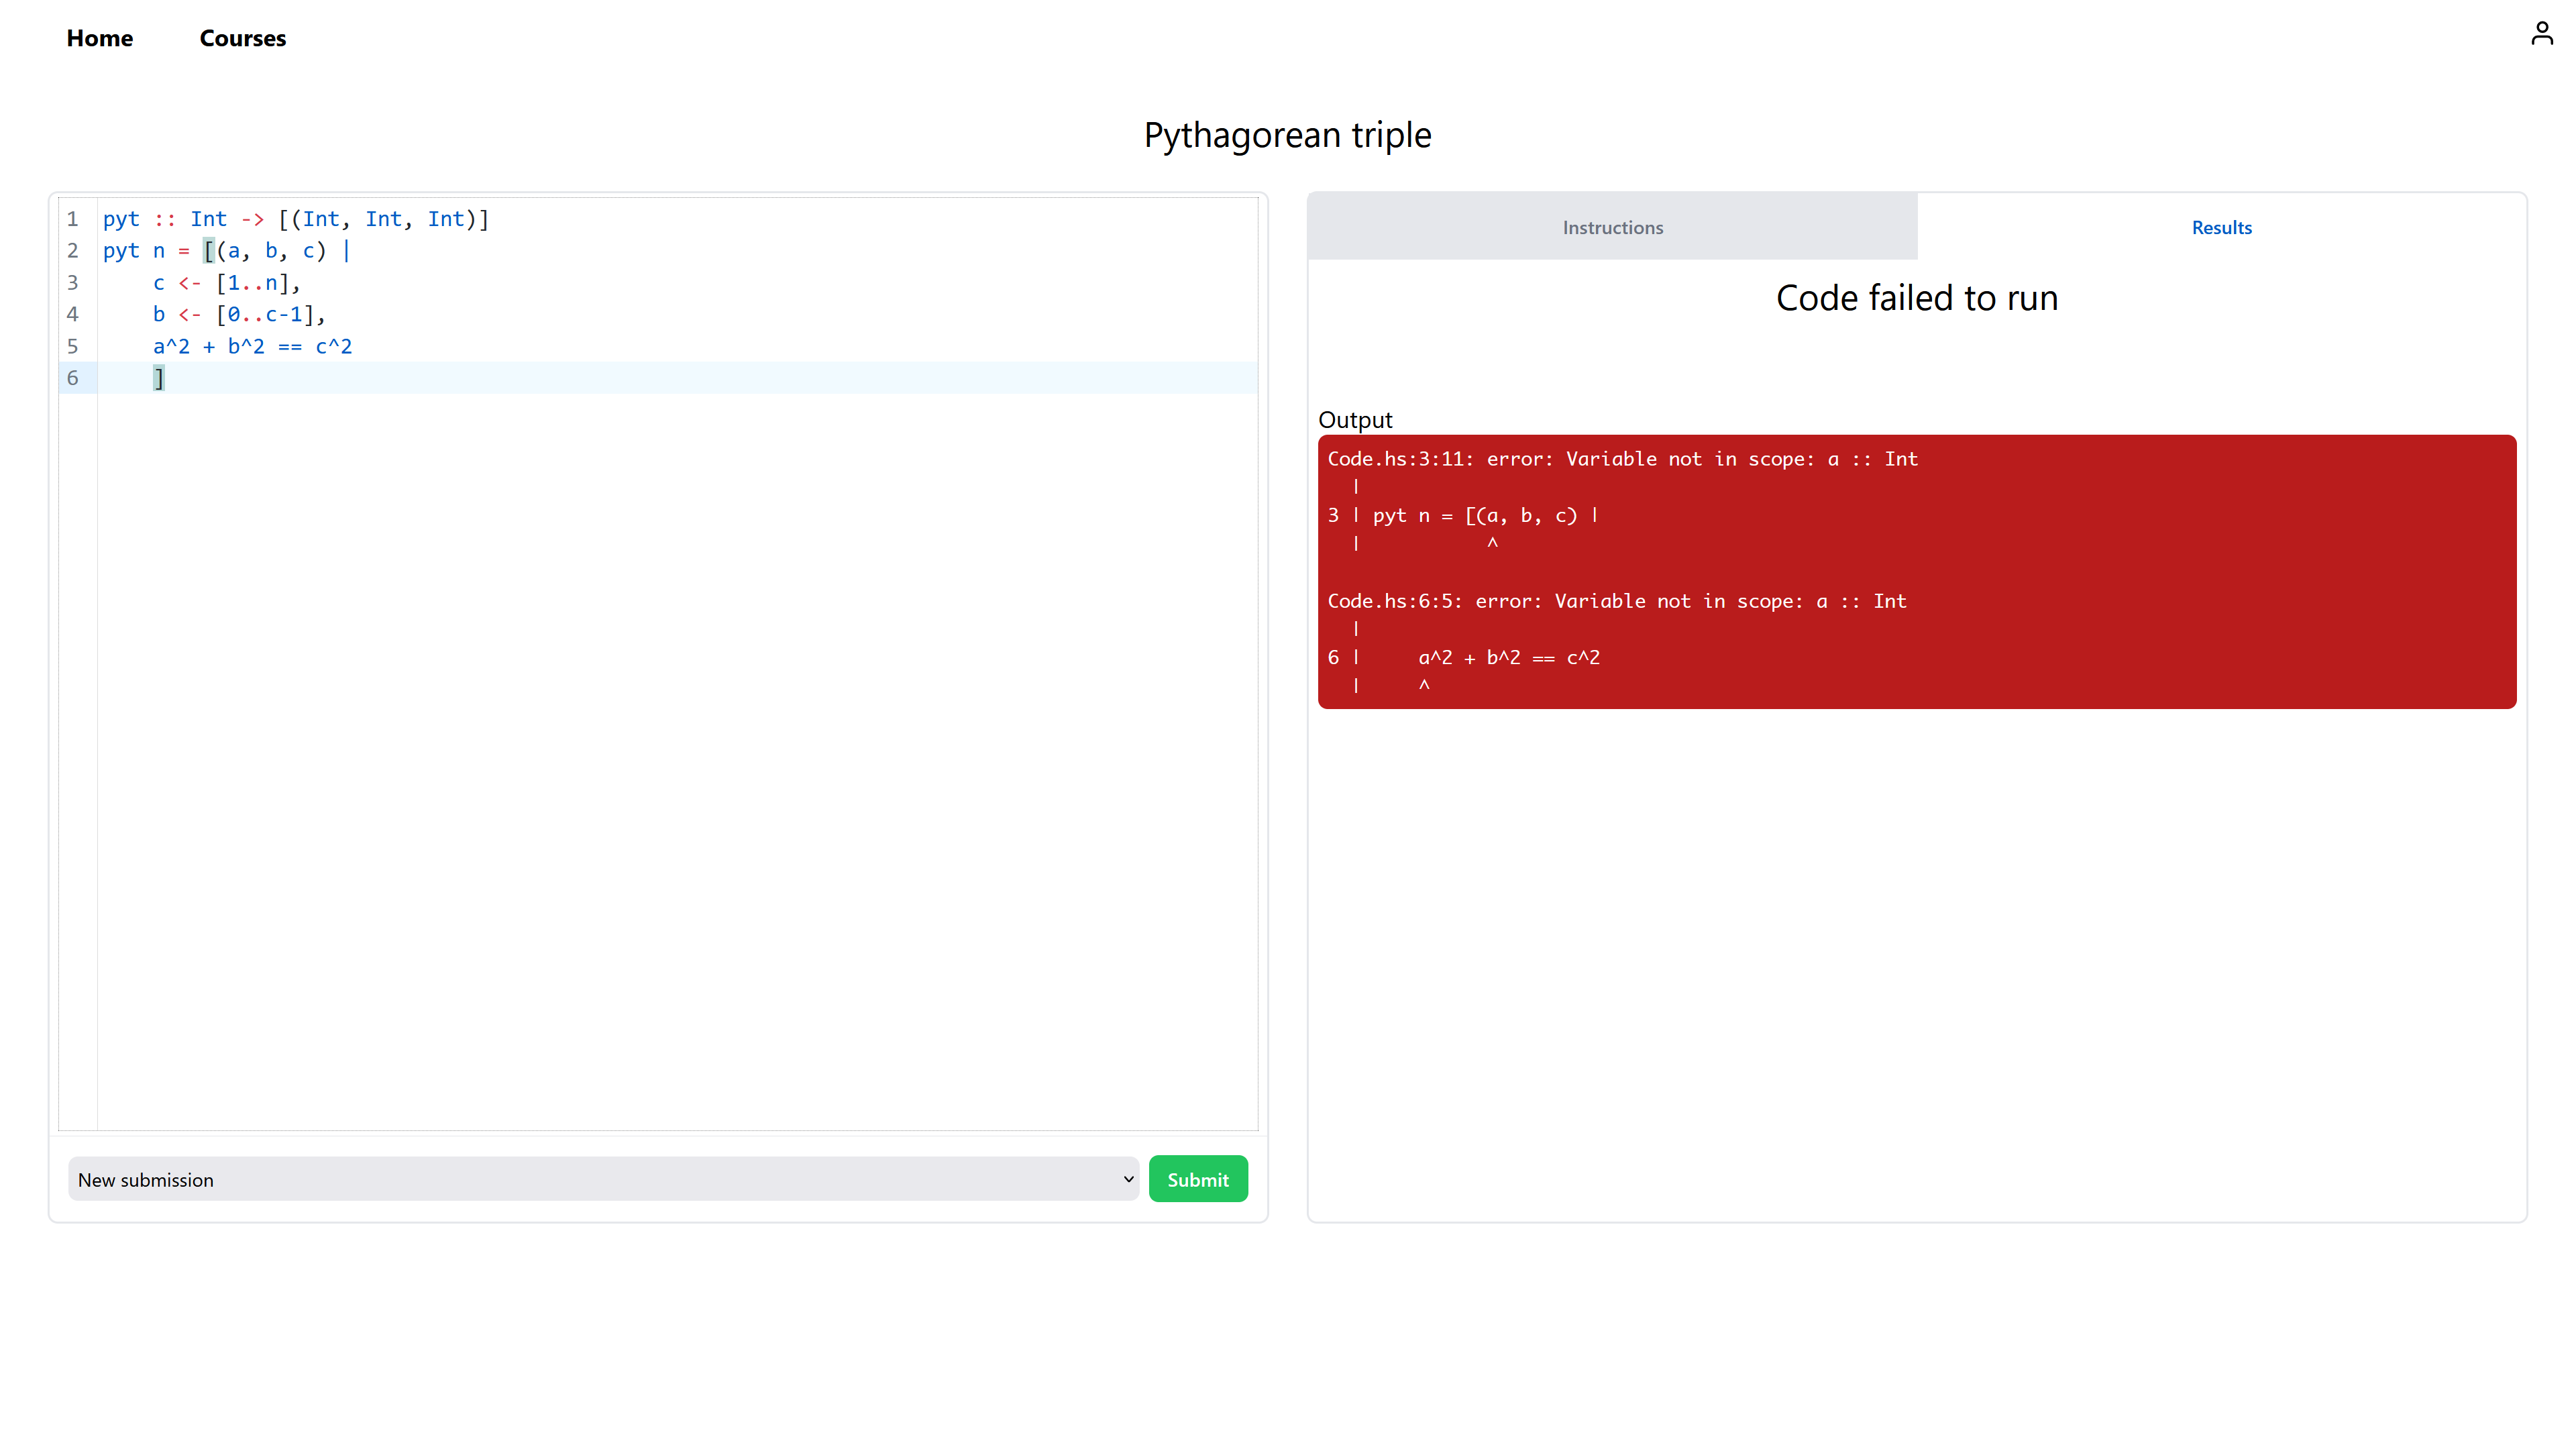
\includegraphics[scale=0.1]{exercise_fail.png}
	\centering
	\caption{An example of an unsuccessful exercise submission}
	\label{fig:exercise_fail}
\end{figure}

More images of the platform user interface can be seen in chapter \ref{chap:images} in the appendix.
